%%%%%%%%%%%%%%%%%%%%%%%%%%%%%%%%%%%%%%%%%%%%%%%%%%%%%%%%%%%%%%%
%% OXFORD THESIS TEMPLATE

% Use this template to produce a standard thesis that meets the Oxford University requirements for DPhil submission
%
% Originally by Keith A. Gillow (gillow@maths.ox.ac.uk), 1997
% Modified by Sam Evans (sam@samuelevansresearch.org), 2007
% Modified by John McManigle (john@oxfordechoes.com), 2015
% Modified by Ulrik Lyngs (ulrik.lyngs@cs.ox.ac.uk), 2018, for use with R Markdown
%
% Ulrik Lyngs, 25 Nov 2018: Following John McManigle, broad permissions are granted to use, modify, and distribute this software
% as specified in the MIT License included in this distribution's LICENSE file.
%
% John tried to comment this file extensively, so read through it to see how to use the various options.  Remember
% that in LaTeX, any line starting with a % is NOT executed.  Several places below, you have a choice of which line to use
% out of multiple options (eg draft vs final, for PDF vs for binding, etc.)  When you pick one, add a % to the beginning of
% the lines you don't want.


%%%%% CHOOSE PAGE LAYOUT
% The most common choices should be below.  You can also do other things, like replacing "a4paper" with "letterpaper", etc.

% This one will format for two-sided binding (ie left and right pages have mirror margins; blank pages inserted where needed):
%\documentclass[a4paper,twoside]{templates/ociamthesis}
% This one will format for one-sided binding (ie left margin > right margin; no extra blank pages):
%\documentclass[a4paper]{ociamthesis}
% This one will format for PDF output (ie equal margins, no extra blank pages):
%\documentclass[a4paper,nobind]{templates/ociamthesis}
%UL 2 Dec 2018: pass this in from YAML
\documentclass[a4paper, nobind]{templates/ociamthesis}


% UL 30 Nov 2018 pandoc puts lists in 'tightlist' command when no space between bullet points in Rmd file
\providecommand{\tightlist}{%
  \setlength{\itemsep}{0pt}\setlength{\parskip}{0pt}}
 
% UL 1 Dec 2018, fix to include code in shaded environments

%UL 2 Dec 2018 reduce whitespace around verbatim environments
\usepackage{etoolbox}
\makeatletter
\preto{\@verbatim}{\topsep=0pt \partopsep=0pt }
\makeatother

%UL 26 Mar 2019, enable strikethrough
\usepackage[normalem]{ulem}

%UL 15 Oct 2019, enable link highlighting to be turned off from YAML
\usepackage[colorlinks=false,pdfpagelabels,hidelinks=true]{hyperref}

%%%%% SELECT YOUR DRAFT OPTIONS
% Three options going on here; use in any combination.  But remember to turn the first two off before
% generating a PDF to send to the printer!

% This adds a "DRAFT" footer to every normal page.  (The first page of each chapter is not a "normal" page.)
\fancyfoot[C]{\emph{DRAFT Printed on \today}}

% This highlights (in blue) corrections marked with (for words) \mccorrect{blah} or (for whole
% paragraphs) \begin{mccorrection} . . . \end{mccorrection}.  This can be useful for sending a PDF of
% your corrected thesis to your examiners for review.  Turn it off, and the blue disappears.
\correctionstrue

%%%%% BIBLIOGRAPHY SETUP
% Note that your bibliography will require some tweaking depending on your department, preferred format, etc.
% The options included below are just very basic "sciencey" and "humanitiesey" options to get started.
% If you've not used LaTeX before, I recommend reading a little about biblatex/biber and getting started with it.
% If you're already a LaTeX pro and are used to natbib or something, modify as necessary.
% Either way, you'll have to choose and configure an appropriate bibliography format...

% The science-type option: numerical in-text citation with references in order of appearance.
% \usepackage[style=numeric-comp, sorting=none, backend=biber, doi=false, isbn=false]{biblatex}
% \newcommand*{\bibtitle}{References}

% The humanities-type option: author-year in-text citation with an alphabetical works cited.
% \usepackage[style=authoryear, sorting=nyt, backend=biber, maxcitenames=2, useprefix, doi=false, isbn=false]{biblatex}
% \newcommand*{\bibtitle}{Works Cited}

%UL 3 Dec 2018: set this from YAML in index.Rmd
\usepackage[style=authoryear, sorting=nyt, backend=biber, maxcitenames=2, useprefix, doi=true, isbn=false, uniquename=false]{biblatex}
\newcommand*{\bibtitle}{Bibliography}

% This makes the bibliography left-aligned (not 'justified') and slightly smaller font.
\renewcommand*{\bibfont}{\raggedright\small}

% Change this to the name of your .bib file (usually exported from a citation manager like Zotero or EndNote).
\addbibresource{bibliography/references.bib}


% Uncomment this if you want equation numbers per section (2.3.12), instead of per chapter (2.18):
%\numberwithin{equation}{subsection}


%%%%% THESIS / TITLE PAGE INFORMATION
% Everybody needs to complete the following:
\title{Lipids and dementia\\
An investigation of their relationship}
\author{Luke A McGuinness}
\college{}

% Master's candidates who require the alternate title page (with candidate number and word count)
% must also un-comment and complete the following three lines:
%\masterssubmissiontrue
%\candidateno{933516}
%\wordcount{28,815}

% Uncomment the following line if your degree also includes exams (eg most masters):
%\renewcommand{\submittedtext}{Submitted in partial completion of the}
% Your full degree name.  (But remember that DPhils aren't "in" anything.  They're just DPhils.)
\degree{Doctor of Philosophy in Population Health Sciences}
% Term and year of submission, or date if your board requires (eg most masters)
\degreedate{TBC}


%%%%% YOUR OWN PERSONAL MACROS
% This is a good place to dump your own LaTeX macros as they come up.

% To make text superscripts shortcuts
	\renewcommand{\th}{\textsuperscript{th}} % ex: I won 4\th place
	\newcommand{\nd}{\textsuperscript{nd}}
	\renewcommand{\st}{\textsuperscript{st}}
	\newcommand{\rd}{\textsuperscript{rd}}

%%%%% THE ACTUAL DOCUMENT STARTS HERE
\begin{document}

%%%%% CHOOSE YOUR LINE SPACING HERE
% This is the official option.  Use it for your submission copy and library copy:
\setlength{\textbaselineskip}{22pt plus2pt}
% This is closer spacing (about 1.5-spaced) that you might prefer for your personal copies:
%\setlength{\textbaselineskip}{18pt plus2pt minus1pt}

% You can set the spacing here for the roman-numbered pages (acknowledgements, table of contents, etc.)
\setlength{\frontmatterbaselineskip}{17pt plus1pt minus1pt}

% UL: You can set the line and paragraph spacing here for the separate abstract page to be handed in to Examination schools
\setlength{\abstractseparatelineskip}{13pt plus1pt minus1pt}
\setlength{\abstractseparateparskip}{0pt plus 1pt}

% UL: You can set the general paragraph spacing here - I've set it to 2pt (was 0) so
% it's less claustrophobic
\setlength{\parskip}{2pt plus 1pt}


% Leave this line alone; it gets things started for the real document.
\setlength{\baselineskip}{\textbaselineskip}


%%%%% CHOOSE YOUR SECTION NUMBERING DEPTH HERE
% You have two choices.  First, how far down are sections numbered?  (Below that, they're named but
% don't get numbers.)  Second, what level of section appears in the table of contents?  These don't have
% to match: you can have numbered sections that don't show up in the ToC, or unnumbered sections that
% do.  Throughout, 0 = chapter; 1 = section; 2 = subsection; 3 = subsubsection, 4 = paragraph...

% The level that gets a number:
\setcounter{secnumdepth}{2}
% The level that shows up in the ToC:
\setcounter{tocdepth}{2}


%%%%% ABSTRACT SEPARATE
% This is used to create the separate, one-page abstract that you are required to hand into the Exam
% Schools.  You can comment it out to generate a PDF for printing or whatnot.
\begin{abstractseparate}
  \textbf{Background}\\
  In the UK, an estimated 800000 people are currently living with dementia and this number is expected to double
  by 2040. Despite the number of dementia cases and decades of research, there remains much unknown about
  the pathogenesis and progression of the disease, and, at present, no effective treatment exists to arrest or
  reverse the cognitive decline associated with the condition. In this context, identification of causal relationships
  between modifiable targets and dementia risk is central to the development of evidence-based prevention
  strategies and will be critically important in maintaining the long-term health of the ageing public. Blood lipid
  levels have been implicated in the aetiology of dementia by genetic linkage and functional cell biology studies,
  but current epidemiological evidence has yet to reach a consensus on their role in dementia risk.
\end{abstractseparate}

% JEM: Pages are roman numbered from here, though page numbers are invisible until ToC.  This is in
% keeping with most typesetting conventions.
\begin{romanpages}

% Title page is created here
\maketitle

%%%%% DEDICATION -- If you'd like one, un-comment the following.
\begin{dedication}
  For Brendan McHugh
\end{dedication}

%%%%% ACKNOWLEDGEMENTS -- Nothing to do here except comment out if you don't want it.
\begin{acknowledgements}
 	This is where you will normally thank your advisor, colleagues, family and friends, as well as funding and institutional support. In our case, we will give our praises to the people who developed the ideas and tools that allow us to push open science a little step forward by writing plain-text, transparent, and reproducible theses in R Markdown.

\begin{flushright}
Luke McGuinness \\
Canynge Hall, Bristol \\
1 December 2021
\end{flushright}
\end{acknowledgements}


%%%%% ABSTRACT -- Nothing to do here except comment out if you don't want it.
\begin{abstract}
	\textbf{Background}\\
In the UK, an estimated 800000 people are currently living with dementia and this number is expected to double
by 2040. Despite the number of dementia cases and decades of research, there remains much unknown about
the pathogenesis and progression of the disease, and, at present, no effective treatment exists to arrest or
reverse the cognitive decline associated with the condition. In this context, identification of causal relationships
between modifiable targets and dementia risk is central to the development of evidence-based prevention
strategies and will be critically important in maintaining the long-term health of the ageing public. Blood lipid
levels have been implicated in the aetiology of dementia by genetic linkage and functional cell biology studies,
but current epidemiological evidence has yet to reach a consensus on their role in dementia risk.
\end{abstract}

%%%%% MINI TABLES
% This lays the groundwork for per-chapter, mini tables of contents.  Comment the following line
% (and remove \minitoc from the chapter files) if you don't want this.  Un-comment either of the
% next two lines if you want a per-chapter list of figures or tables.
  \dominitoc % include a mini table of contents

% This aligns the bottom of the text of each page.  It generally makes things look better.
\flushbottom

% This is where the whole-document ToC appears:
\tableofcontents

\listoffigures
	\mtcaddchapter
  	% \mtcaddchapter is needed when adding a non-chapter (but chapter-like) entity to avoid confusing minitoc

% Uncomment to generate a list of tables:
\listoftables
  \mtcaddchapter
%%%%% LIST OF ABBREVIATIONS
% This example includes a list of abbreviations.  Look at text/abbreviations.tex to see how that file is
% formatted.  The template can handle any kind of list though, so this might be a good place for a
% glossary, etc.
% First parameter can be changed eg to "Glossary" or something.
% Second parameter is the max length of bold terms.
\begin{mclistof}{List of Abbreviations}{3.2cm}

\item[1-D, 2-D] One- or two-dimensional, referring in this thesis to spatial dimensions in an image.

\item[Otter] One of the finest of water mammals.

\item[Hedgehog] Quite a nice prickly friend.

\end{mclistof} 


% The Roman pages, like the Roman Empire, must come to its inevitable close.
\end{romanpages}

%%%%% CHAPTERS
% Add or remove any chapters you'd like here, by file name (excluding '.tex'):
\flushbottom

% all your chapters and appendices will appear here
\hypertarget{covering-material}{%
\chapter*{Covering material}\label{covering-material}}
\addcontentsline{toc}{chapter}{Covering material}

\adjustmtc

\begin{verbatim}
## For information on available language packages for 'koRpus', run
## 
##   available.koRpus.lang()
## 
## and see ?install.koRpus.lang()
\end{verbatim}

Word count: 1163

\hypertarget{intro-intro}{%
\chapter{Introduction}\label{intro-intro}}

\minitoc 

This is a test of the bibliography\textsuperscript{\protect\hyperlink{ref-chang2012}{1}}

The following tools were used to perform the risk of bias assessments: ROB-2, ROBINS-I and QUADAS-2

\begin{savequote}
Hold
\qauthor{--- Charles Darwin\textsuperscript{\protect\hyperlink{ref-chang2012}{1}}}\end{savequote}



\hypertarget{chapter-2-headings}{%
\chapter{Chapter 2: Systematic Review}\label{chapter-2-headings}}

\minitoc 

\hypertarget{aims}{%
\section{Aims}\label{aims}}

The aim of this chapter is to systematically review all available literature on the association between blood levels of total cholesterol and it's constituent parts (HDL-c,LDL-c and triglycerides) on the subsequent risk of dementia.

\hypertarget{methods}{%
\section{Methods}\label{methods}}

\hypertarget{search-strategy}{%
\subsection{Search strategy}\label{search-strategy}}

We will systematically search electronic bibliographic databases to identify potentially relevant records. The search strategy used in each database will be developed in an iterative manner using a combination of free text and controlled vocabulary (MeSH/EMTREE) terms to identify studies which have examined the relationship between blood lipids levels and dementia, incorporating input from an information specialist. The strategy will include terms related to lipids, lipid modifying treatments, and dementia and its sub-types, and will be designed for MEDLINE before being adapted for use in the other bibliography databases listed. An outline of the general strategy is presented in the Table 3.2 below and the full draft search strategies for each database are attached to this protocol. To ensure that the study design filters are not excluding potentially relevant records, a random sample of 500 records identified by the main search but excluded by the filters (defined as Line 7 NOT Line 13 in Table 3.2) will be screened. If any potentially relevant studies are identified, their titles and abstracts will be searched for key terms that can be incorporated into the filters to improve search sensitivity.

The following databases will be searched from inception onwards: Medline, EMBASE, Psychinfo, Cochrane Central Register of Controlled Trials (CENTRAL), and Web of Science Core Collection. We will also search clinical trial registries, for example ClinicalTrials.gov, to identify relevant randomized controlled trials.

The abstracts list of relevant conferences (e.g.~the proceedings of the Alzheimer's Association International Conference, published in the journal Alzheimer's \& Dementia) will be searched. Grey literature will also be searched via ProQuest, OpenGrey and Web of Science Conference Proceedings Citation Index, while theses will be accessed using the Open Access Theses and Dissertations portal. We will also search BioArxiv, a preprint repository, to identify potentially relevant studies. Finally, the reference lists of included studies will be searched by hand while studies citing included studies will be examined using Google Scholar (forward and reverse citation searching).

\hypertarget{study-selection}{%
\subsection{Study selection}\label{study-selection}}

Records will be imported into Endnote and deduplicated using the method outlined in Bramer et al.~(2016).\textsuperscript{\protect\hyperlink{ref-bramer2016}{2}} Screening (both title/abstract and full-text) will be performed using a combination of Endnote and Rayyan, a web based screening application.\textsuperscript{\protect\hyperlink{ref-ouzzani2016}{3}}
Title and abstract screening to remove obviously irrelevant records will be performed by the primary author, with a random selection of excluded records being screened in duplicate to ensure consistency with the inclusion criteria. If this demonstrates a significant level of erroneous exclusion by the primary author a larger proportion will be dual-screened.
Full-text screening will also be completed in full by the primary author. A second reviewer will screen a random sample of included and excluded records, in addition to any records identified by the first reviewer as being difficult to assess against the inclusion criteria. Reasons for exclusion at this stage will be recorded. Disagreements occurring during either stage of the screening process will be resolved through discussion with a senior colleague. A PRIMSA flow diagram will be produced to document how records moved through the review.\textsuperscript{\protect\hyperlink{ref-zotero-766}{4}}

\hypertarget{inclusion}{%
\subsubsection{Inclusion}\label{inclusion}}

We will seek studies that examine the relationship between blood lipid levels (or any specific lipid fraction, including total cholesterol, HDL, LDL, and triglycerides) and risk of incident dementia/MCI. Eligible study designs include randomized controlled trials and non-randomized observational studies of lipid modifying treatments, longitudinal studies examining the effect of increased/decreased blood lipid levels, and genetic instrumental variable (Mendelian randomization) studies examining the effect of genetically increased/decreased blood lipid levels.

Participants will be free (or assumed to be free) of dementia/MCI at baseline. Studies of any duration will be included to allow for exploration of the effect of length of follow-up on the effect estimate using meta-regression. No limits will be placed on the sample size of included studies.

Eligible studies will define dementia according to recognised criteria, for example the National Institute of Neurological Disorders and Stroke Association-Internationale pour la Recherche en l'Enseignement en Neurosciences (NINDS-AIREN), International Classification of Diseases (ICD), or Diagnostic and Statistical Manual of Mental Disorders (DSM) criteria. For MCI, eligible studies are those that attempted state a definition for diagnoses of MCI (e.g.~an adapted version of the Petersen criteria\textsuperscript{\protect\hyperlink{ref-petersen1999}{5}}) and create ordinal groups of patients (e.g.~no dementia or dementia/MCI/dementia) based on this definition.

No limitations will be imposed on publication status, publication date, venue or language, although we will require sufficiently detailed reports of the studies to be able to examine their methods. Preprints and unpublished reports will be eligible for inclusion if relevant. Multiple publications resulting from the analysis of the same data will be included and grouped.

\hypertarget{exclusion}{%
\subsubsection{Exclusion}\label{exclusion}}

Case-control studies, cross-sectional studies, qualitative studies, case reports/series and narrative reviews will be excluded. Studies which present no evidence of attempting to exclude prevalent cases from their analyses will also be excluded. Studies that measure change in continuous cognitive measures (e.g.~MoCA score) without attempt to map these scores to ordinal groups (e.g.~no dementia/MCI/dementia) will be excluded. Conference abstracts with no corresponding full-text publication will be examined, and we will contact authors to obtain information on the study's status. Studies that are reported in insufficient detail (e.g.~only in conference abstracts, new, letters, editorials and opinion) will be excluded. Previous systematic reviews will not be eligible, but their reference lists will be screened to identify any potentially relevant articles. Studies with outcomes not directly related to the clinical syndrome of dementia (e.g., neuroimaging), studies implementing a ``multidomain intervention'' where the lipid-regulating agent is included in each arms (e.g.~for example, a study examining exercise + statins vs statins alone, but a study examining exercise + statins vs exercise alone would be included), and studies where there was no screening for dementia at baseline except if the sample was initially assessed in mid-life (i.e.~below the age of 50) will be excluded.

\hypertarget{data-extraction}{%
\subsection{Data extraction}\label{data-extraction}}

\hypertarget{risk-of-bias-assessment}{%
\subsection{Risk of bias assessment}\label{risk-of-bias-assessment}}

Risk of bias assessment was performed using the domain-based risk-of-bias assessment tool appropriate to the study design. Randomised controlled trials were assessed using the RoB2 tool,\textsuperscript{\protect\hyperlink{ref-sterne2019}{6}}, non-randomised studies of interventions were assessed using the ROBINS-I tool,\textsuperscript{\protect\hyperlink{ref-sterne2016}{7}} and non-randomised studies of exposures were assessed using the ROBINS-E tool.{[}TBC{]}

At present, no risk of bias assessment tool for Mendelian randomisation studies is available. Bias in thesee studies was assessed with the help of an expert panel {[}TBC{]}

\hypertarget{patient-and-public-involvement}{%
\subsection{Patient and public involvement}\label{patient-and-public-involvement}}

\hypertarget{results}{%
\section{Results}\label{results}}

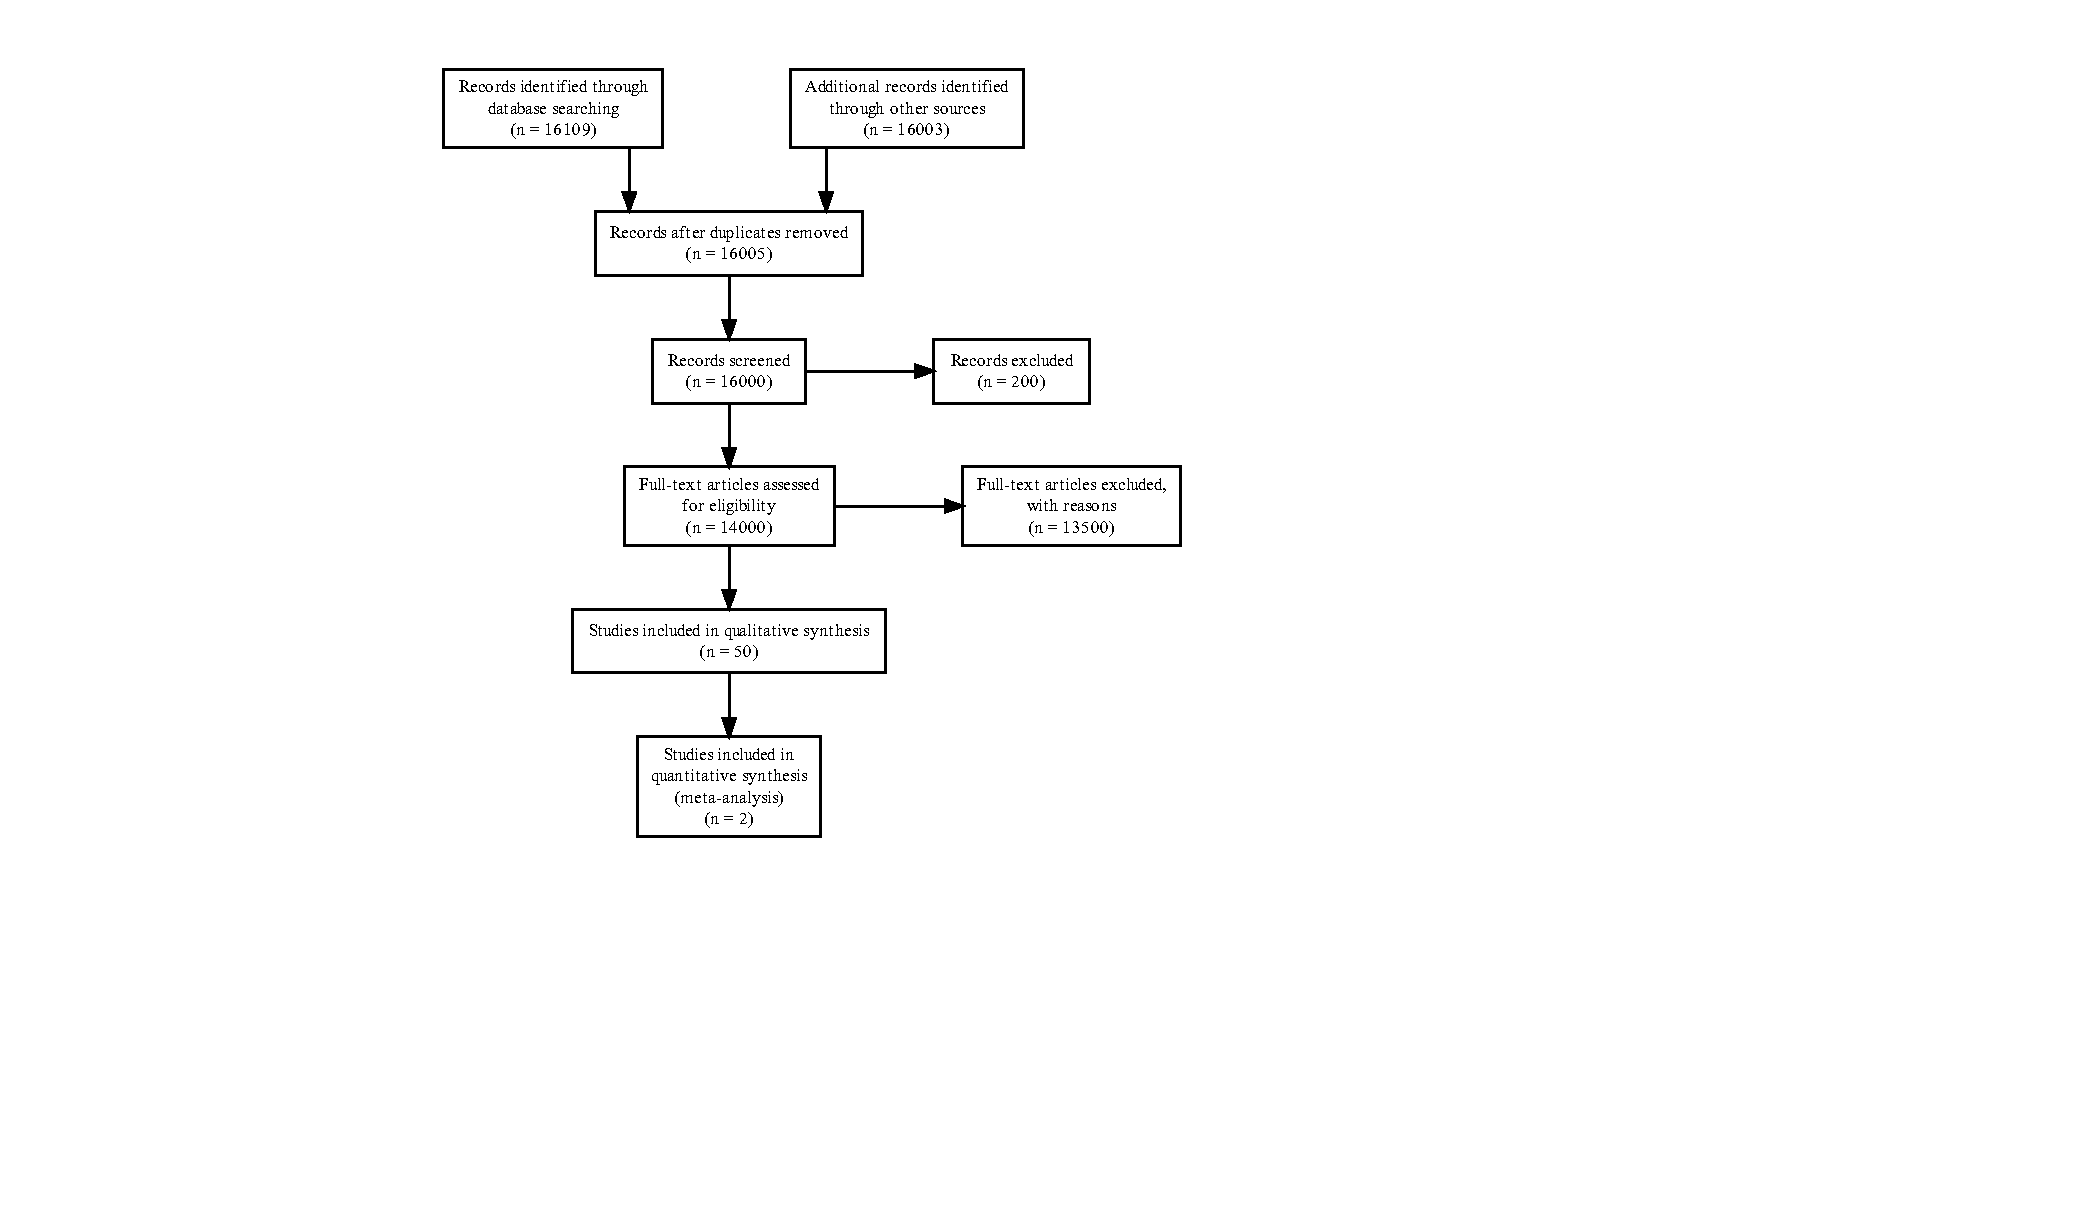
\includegraphics{_main_files/figure-latex/prisma-flow-1.pdf}

\hypertarget{discussion}{%
\section{Discussion}\label{discussion}}

\hypertarget{conclusion}{%
\section{Conclusion}\label{conclusion}}

\hypertarget{annotated-bibliography}{%
\chapter{Annotated Bibliography}\label{annotated-bibliography}}

\startappendices

\hypertarget{list-of-one-thing}{%
\chapter{List of one thing}\label{list-of-one-thing}}

\hypertarget{list-of-something-else}{%
\chapter{List of something else}\label{list-of-something-else}}

\hypertarget{refs}{}
\leavevmode\hypertarget{ref-chang2012}{}%
1. Chang, C.-C. H., Zhao, Y., Lee, C.-W. \& Ganguli, M. Smoking, death, and Alzheimer's disease: A case of competing risks. \emph{Alzheimer Disease and Associated Disorders} \textbf{26}, 300--306 (2012).

\leavevmode\hypertarget{ref-bramer2016}{}%
2. Bramer, W. M., Giustini, D., de Jonge, G. B., Holland, L. \& Bekhuis, T. De-duplication of database search results for systematic reviews in EndNote. \emph{Journal of the Medical Library Association : JMLA} \textbf{104}, 240--243 (2016).

\leavevmode\hypertarget{ref-ouzzani2016}{}%
3. Ouzzani, M., Hammady, H., Fedorowicz, Z. \& Elmagarmid, A. Rayyan-a web and mobile app for systematic reviews. \emph{Systematic Reviews} \textbf{5}, 210 (2016).

\leavevmode\hypertarget{ref-zotero-766}{}%
4. The PRISMA statement for reporting systematic reviews and meta-analyses of studies that evaluate healthcare interventions: Explanation and elaboration \textbar{} The BMJ.

\leavevmode\hypertarget{ref-petersen1999}{}%
5. Petersen, R. C. \emph{et al.} Mild cognitive impairment: Clinical characterization and outcome. \emph{Archives of Neurology} \textbf{56}, 303--308 (1999).

\leavevmode\hypertarget{ref-sterne2019}{}%
6. Sterne, J. A. C. \emph{et al.} RoB 2: A revised tool for assessing risk of bias in randomised trials. \emph{BMJ} \textbf{366}, (2019).

\leavevmode\hypertarget{ref-sterne2016}{}%
7. Sterne, J. A. \emph{et al.} ROBINS-I: A tool for assessing risk of bias in non-randomised studies of interventions. \emph{BMJ} \textbf{355}, (2016).


%%%%% REFERENCES

% JEM: Quote for the top of references (just like a chapter quote if you're using them).  Comment to skip.
% \begin{savequote}[8cm]
% The first kind of intellectual and artistic personality belongs to the hedgehogs, the second to the foxes \dots
%   \qauthor{--- Sir Isaiah Berlin \cite{berlin_hedgehog_2013}}
% \end{savequote}

\setlength{\baselineskip}{0pt} % JEM: Single-space References

{\renewcommand*\MakeUppercase[1]{#1}%
\printbibliography[heading=bibintoc,title={\bibtitle}]}

\end{document}
